%
\documentclass{ar-1col}
\usepackage{cite}
\usepackage{xspace}
\usepackage{url}
\usepackage{slashed}
\usepackage{soul,upgreek}
\usepackage{amssymb}

% Definitions
\newcommand{\chiDM}{\ensuremath{\chi}\xspace}
%\newcommand{\IP}{\ensuremath{\textrm{IP}}\xspace}
\newcommand{\IP}{invisible particle}
\newcommand{\mMed}{\ensuremath{M_{\rm{med}}}\xspace}
\newcommand{\mmed}{\mMed}
\newcommand{\gDM}{\ensuremath{g_{\chiDM}}\xspace}
\newcommand{\gdm}{\gDM}
\newcommand{\gl}{$g_{\ell}$\xspace}
\newcommand{\gdmq}{\ensuremath{g_{\chiDM q}}\xspace}
\newcommand{\gq}{$g_{\mathrm{q}}$\xspace}
%\newcommand{\ifb}{\ensuremath{\mathrm{fb}^{-1}}\xspace}
\newcommand{\mdm}{\ensuremath{m_{\chiDM}}\xspace}
\newcommand{\mDM}{\mdm}
\newcommand{\ghZprimeZprime}{\ensuremath{g_{hZ'Z'}}\xspace}
\newcommand{\gZPrime}{\ensuremath{g_{Z'}}\xspace}
\newcommand{\gZprime}{\ensuremath{g_{Z'}}\xspace}
\newcommand{\sinthetab}{\ensuremath{\mathrm{sin}(\theta_B})\xspace}
\newcommand{\sinthetahS}{\ensuremath{\mathrm{sin}(\theta_{hS})}\xspace}
\newcommand{\pt}{\ensuremath{p_\mathrm{T}}\xspace}
\newcommand{\pT}{\ensuremath{p_\mathrm{T}}\xspace}
\newcommand{\MET}{\ensuremath{\slashed{E}_T}\xspace}
\newcommand{\Zprime}{\ensuremath{{Z}^\prime}\xspace}
\newcommand{\fb}{\ensuremath{\mathrm{fb}}\xspace}
\newcommand{\pb}{\ensuremath{\mathrm{pb}}\xspace}
\newcommand{\ifb}{\ensuremath{\mathrm{fb}^{-1}}\xspace}
\newcommand{\ipb}{\ensuremath{\mathrm{pb}^{-1}}\xspace}
\setcounter{secnumdepth}{4}

% Metadata Information
\jname{Annu. Rev. Nucl. Part. Sci.} \jvol{68} \jyear{2018}
\doi{10.1146/annurev-nucl-101917-021008}

\begin{document}

\markboth{Boveia $\bullet$ Doglioni}{Dark Matter Searches at Colliders}

\title{Dark Matter Searches at Colliders}

\author{Antonio Boveia$^1$ and Caterina Doglioni$^2$
\affil{$^1$Physics Department, The Ohio State University, Columbus, Ohio 43210, USA} \affil{$^2$Fysikum, Division of Particle Physics, Lund
University, 22363 Lund, Sweden}}

\clearpage

\begin{figure}[!htpb]
\includegraphics[width=\textwidth]{figs_standalone/feynman_0}
\caption{(\textit{a}) The interaction between DM\ and Standard Model particles via an unspecified interaction (e.g., an EFT).
(\textit{b}) Examples of simplified model processes where the interaction is mediated by an intermediate particle (with additional radiation off one of the initial-state quarks). 
(\textit{c}) The same model, in which  the mediator decays back into Standard Model particles, with coupling constant  \gq  for the mediator--quark--quark vertex and constant  \gdm for the mediator--DM vertex. 
Abbreviations:\ BSM, beyond the Standard Model; DM, dark matter; EFT, effective field theory; SM, Standard Model. \label{fig:feynman_0}}
\end{figure}

\clearpage

\begin{figure}[!htpb]
\includegraphics[width=\textwidth]{figs_standalone/feynman_1}
\caption{
(\textit{a}) Example of a process including baryonic coupling between a vector mediator $Z'$ and an SM Higgs boson. The $Z'$--Higgs coupling is denoted \ghZprimeZprime. 
(\textit{b}) Example of a process from a \textit{U}(1) $Z'$ boson embedded in a 2HDM, where a vector $Z'$ decays to a pseudoscalar $A^0$ that in turn decays to DM particles. 
(\textit{c,d}) Examples of a simplified model process where the interaction is mediated by an intermediate scalar or pseudoscalar particle. In panel \textit{c}, the SM--scalar interaction proceeds through a gluon loop \cite{Haisch:2013ata}, whereas in panel \textit{d}, the pseudo(scalar) is produced in association with a pair of heavy-flavor quarks. The coupling constants that are prefactors to the Yukawa couplings in the model are denoted \gq for the mediator--quark--quark vertex and \gdm for the mediator--DM vertex. 
Abbreviations:\ $A^0/a$, pseudoscalar bosons; $b$, bottom quark; DM, dark matter;  $g$, gluon; $h$, SM Higgs boson; $S$, heavy scalar boson; SM, Standard Model; $t$, top quark; $Z'$, vector mediator; 2HDM, two--Higgs doublet model. }
\label{fig:feynman_1}
\end{figure}

\clearpage

\begin{figure}[!htpb]
\includegraphics[width=\textwidth]{figs_standalone/feynman_2}
\caption{
(\textit{a}) Example of a process leading to a single top signature, proceeding through the coupling of a $u$ and a $t$ with a new vector boson, decaying to DM particles. 
(\textit{b}) Example of a collider diagram from a coannihilation model, where two DM particles are present in the final state (one denoted DM and the other  $X$). 
(\textit{c}) Example of a diagram from a 2HDM process, with an interaction between an  $H$, an SM $Z$ boson, and an $a$ mediating the SM--DM interaction. 
Abbreviations:\ $a$, pseudoscalar boson; DM, dark matter; $g$, gluon; $H$, heavy Higgs boson; SM, Standard Model; $t$, top quark;  $u$, up quark; $V$, vector mediator; $X$, coannihilating DM partner, 2HDM, two--Higgs doublet model.}
\label{fig:feynman_2}
\end{figure}

\clearpage

\begin{figure}[!htpb]
\includegraphics[width=0.5\textwidth]{figs_standalone/FakeMET}
\caption{The \MET distribution of events, termed as $E_T^{miss}$ in the x axis, selected for high total
hadronic energy and at least two jets with \pt{} $>$ 400 and 200
GeV, before (\textit{open circles}) and after (\textit{filled circles}) rejection of
spurious \MET backgrounds~\cite{CMS-PAS-JME-16-004}. The
predictions of Monte Carlo  simulations (\textit{shaded areas}) are also shown. Strong
noncollision background suppression is vital to \textit{X}+\MET analyses.}
\label{fig:fakeMET}
\end{figure}

\clearpage

\begin{figure}[!htpb]
\includegraphics[width=\textwidth]{figs_standalone/CMS-SUS-17-004_Figure_010-a.pdf}
\includegraphics[width=\textwidth]{figs_standalone/ATLAS_SUSY_EWSummary_higgsino.pdf}
\caption{Mass reach of (\textit{a})\ CMS and (\textit{b})\ ATLAS searches for a selection of
results targeting electroweak supersymmetry production, available as of
July 2018.
Panel \textit{a} adapted from Reference \citen{Sirunyan:2018ubx}. 
Panel \textit{b} adapted from Reference~\citen{ATL-PHYS-PUB-2017-019}.\label{fig:SUSYSummary_ew}}
\end{figure}

\clearpage

\begin{figure}[!htpb]
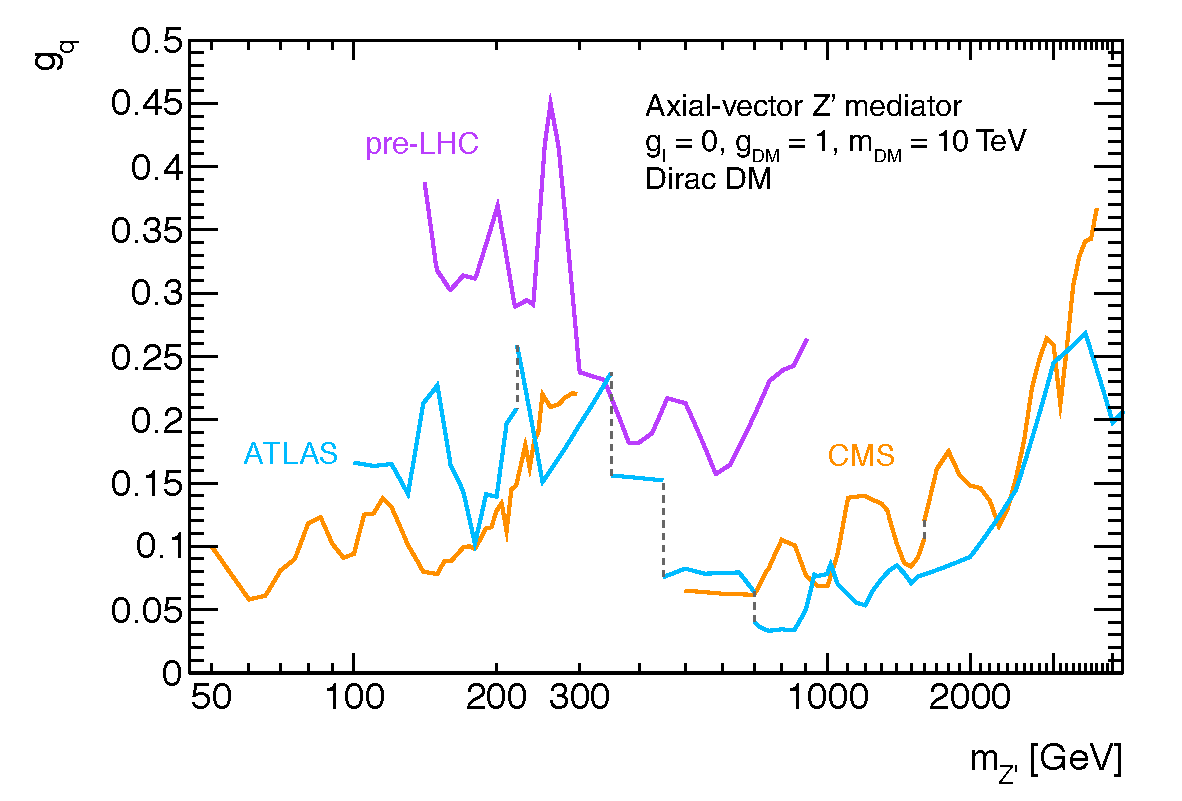
\includegraphics[width=\textwidth]{figs_standalone/CouplingMassPlot.pdf}
\caption{Summary of constraints from searches for narrow, light dijet
resonances from ATLAS and CMS available as of
July 2018, where discrete points are taken
from the coupling-mass limits on a simplified model mediated by an
axial--vector $Z^\prime$ coupling exclusively to quarks from the
searches mentioned in the text, and interpolated at the crossings.
Couplings above the lines are excluded at 95\% CL, up to the
values where larger couplings yield a resonance width larger than
10-15\% (roughly \gq $>$ 0.5). Abbreviation:\ DM, dark matter.
Pre-LHC constraints are extracted from Reference \citen{Dobrescu:2013coa},
while LHC constraints are taken from References \cite{Sirunyan:2017nvi,Aaboud:2018zba,
ATLAS:2016bvn,Sirunyan:2017nvi,Sirunyan:2018xlo,Aaboud:2018fzt,Aaboud:2017yvp}.}
\label{fig:couplingmass}
\end{figure}

\clearpage


\begin{figure}[!htpb]
\includegraphics[width=0.7\textwidth]{figs_standalone/ATLAS_DarkMatter_Summary_Vector.pdf}\\
\includegraphics[width=0.7\textwidth]{figs_standalone/ATLAS_DarkMatter_Summary_Vector_ModifiedCoupling.pdf}
\caption{Regions in DM mass--\Zprime mediator mass
excluded at 95\% CL by a selection of ATLAS searches 
(from References \cite{ATLAS:2016bvn,Aaboud:2018fzt,Aaboud:2017yvp,
Aaboud:2017phn,ATLAS-CONF-2018-005,Aaboud:2017bja,Aaboud:2017dor,
Aaboud:2017buh}) 
available as of July 2018, for two coupling scenarios. Dashed curves labeled ``thermal
relic'' indicate combinations of DM and mediator mass
that are consistent with a DM density of $\omega_c = 0.12
h^2$ and a standard thermal history, as computed in MadDM for this
model~\cite{Backovic:2015cra}. The dotted curve indicates the
kinematic threshold where the mediator can decay on-shell into
DM. 
In panel (a), the couplings of the mediator particle to each generation
of quarks (\gq) are set to 0.25, the couplings to leptons (\gl)
are set to zero and the coupling to DM is set to unity. 
In panel (b), \gq is set to 0.1, \gl is set to 0.01
and the coupling to DM \gdm is set to unity and marked as $g_{DM}$ in this plot.
Abbreviations:\ DM, dark matter; ISR, initial-state radiation; 
TLA, trigger-object level analysis. Adapted from~Reference \citen{ATLASSummary}.
}
\label{fig:sensitivityComparison}
\end{figure}

\clearpage

\begin{figure}[!htpb]
\includegraphics[width=0.9\textwidth]{figs_standalone/SI_CMSDD_Summary}
\caption{The 90\%-CL constraints from the CMS experiment 
from References \cite{Sirunyan:2017nvi,Sirunyan:2018xlo,Sirunyan:2017jix,CMS-PAS-EXO-16-053,Sirunyan:2017qfc}
in the \mdm-spin-independent DM--nucleon plane for a vector mediator,
Dirac DM, and benchmark couplings \gq = 0.25 and \gdm = 1.0 (marked as $g_{DM}$ in this plot) chosen as an example of what
early LHC searches would be sensitive to, compared with direct detection
experiments from References \cite{Angloher:2015ewa,Agnese:2015nto,Cui:2017nnn,Akerib:2016vxi,Aprile:2018dbl}. 
It is important to note that this comparison is only valid for this particular
combination of model and parameter choices. 
Abbreviation:\ DM, dark matter. Adapted from Reference~\citen{CMSSummary}.} \label{fig:SICMS}
\end{figure}



\begin{thebibliography}{175}
\expandafter\ifx\csname
natexlab\endcsname\relax\def\natexlab#1{#1}\fi

\bibitem{Bertone:2004pz}
Bertone G, Hooper D, Silk J. \textit{Phys.\ Rep.}\  {405}:279 (2005) 

\bibitem{Cohen:2016uyg}
  Cohen T, et al. \textit{Phys.\ Rev.\ Lett.}\  {119}:021102 (2017)
  
\bibitem{Ellis:1999mm}
Ellis JR, Falk T, Olive KA, Srednicki M. \textit{Astropart. Phys.}
13:181 (2000); Erratum. \textit{Astropart. Phys.} 15:413 (2001)

\bibitem{Ade:2015xua}
Ade PAR, et~al. \textit{Astron. Astrophys.} 594:A13 (2016)

\bibitem{0954-3899-43-1-013001}
Undagoitia TM, Rauch L. \textit{J. Phys. G}
43:013001 (2016)

\bibitem{Gaskins:2016cha}
Gaskins JM. \textit{Contemp. Phys.} 57:496 (2016)

\bibitem{ATLAS2008}
{{ATLAS Collab.}} \textit{{J. Instrum.}} 3:{S08003} (2008)

\bibitem{CMS2008}
{{CMS Collab.}} \textit{{J. Instrum.}} 3:{S08004} (2008)

\bibitem{LHCb2008}
{{LHCb Collab.}} \textit{{J. Instrum.}} 3:{S08005} (2008)

\bibitem{Steigman:2012nb} 
  Steigman G, Dasgupta B,~Beacom JF. \textit{Phys.\ Rev.\ D} {86}:023506 (2012)

\bibitem{Bernal:2017kxu}
Bernal N, et~al. \textit{Int. J. Mod. Phys.} \textit{A} 32:1730023 (2017)

\bibitem{Brooijmans:2018xbu} 
  Brooijmans G, {et al.} arXiv:1803.10379 [hep-ph] (2018)

\bibitem{Evans:2017kti}
Evans JA, Gori S, Shelton J. \textit{J. High Energy Phys.} {1802}:100 (2018)

\bibitem{DAmbrosio:2002vsn}
D'Ambrosio G, Giudice GF, Isidori G, Strumia A. \textit{Nucl.
Phys.} \textit{B} 645:155 (2002)

\bibitem{Abercrombie:2015wmb}
Abercrombie D, et~al. arXiv:1507.00966 [hep-ex] (2015)

\bibitem{Patt:2006fw}
Patt B, Wilczek F. arXiv:hep-ph/0605188 (2006)

\bibitem{Djouadi:2011aa}
Djouadi A, Lebedev O, Mambrini Y, Quevillon J. \textit{Phys.
Lett.} \textit{B} 709:65 (2012)


\bibitem{Escudero:2016gzx}
Escudero M, Berlin A, Hooper D, Lin MX. \textit{J. Cosmol. Astropart. Phys.} 1612:029
(2016)

\bibitem{Goodman:2010ku}
Goodman J, et~al. \textit{Phys. Rev.} \textit{D} 82:116010 (2010)

\bibitem{Bai:2010hh}
Bai Y, Fox PJ, Harnik R. \textit{J. High Energy Phys.} 1012:048 (2010)

\bibitem{Fox:2011pm}
Fox PJ, Harnik R, Kopp J, Tsai Y. \textit{Phys. Rev.} \textit{D} 85:056011
(2012)

\bibitem{Beltran:2010ww} 
  Beltran M, et al.
\textit{J. High Energy Phys.}\ {1009}:037 (2010)

\bibitem{Shoemaker:2011vi}
Shoemaker IM, Vecchi L. \textit{Phys. Rev.} \textit{D} 86:015023 (2012)

\bibitem{Racco:2015dxa}
Racco D, Wulzer A, Zwirner F. \textit{J. High Energy Phys.} 1505:009 (2015)

\bibitem{Busoni:2013lha}
Busoni G, De~Simone A, Morgante E, Riotto A. \textit{Phys. Lett.}
\textit{B} 728:412 (2014)



\bibitem{Alwall:2008ag}
Alwall J, Schuster P, Toro N. \textit{Phys. Rev.} \textit{D} 79:075020
(2009)

\bibitem{Alves:2011wf}
{LHC New Phys. Work. Group}. \textit{J. Phys.} \textit{G} 39:105005
(2012)

\bibitem{DiFranzo:2013vra} 
  DiFranzo A, Nagao KI, Rajaraman A, Tait TMP.
  \textit{J. High Energy Phys.} {1311}:014 (2013);
  Erratum. \textit{J. High Energy Phys.} {1401}:162 (2014)

\bibitem{Abdallah:2015ter}
Abdallah J, et~al. \textit{Phys. Dark Univ.} 9/10:8 (2015)

\bibitem{Kahlhoefer:2015bea}
Kahlhoefer F, Schmidt-Hoberg K, Schwetz T, Vogl S. \textit{J. High Energy Phys.}
02:016 (2016)
\bibitem{Backovic:2015soa}
Backovic M, et~al. \textit{Eur. Phys. J.} \textit{C} 75:482 (2015)

\bibitem{Papucci:2014iwa}
Papucci M, Vichi A, Zurek KM. \textit{J. High Energy Phys.} 1411:024 (2014)

\bibitem{An:2013xka}
An H, Wang LT, Zhang H. \textit{Phys. Rev.} \textit{D} 89:115014 (2014)

\bibitem{Bell:2012rg}
Bell NF, et~al. \textit{Phys. Rev.} \textit{D} 86:096011 (2012)

\bibitem{Han:2015cty}
Han C, Lee HM, Park M, Sanz V. \textit{Phys. Lett.} \textit{B} 755:371
(2016)

\bibitem{Albert:2017onk}
Albert A, et~al. arXiv:1703.05703 [hep-ex] (2017)

\bibitem{Berlin:2014cfa}
Berlin A, Lin T, Wang LT. \textit{J. High Energy Phys.} 1406:078 (2014)

\bibitem{Carpenter:2013xra} 
Carpenter L, et~al. \textit{Phys.\ Rev.\ D} 89:075017 (2014)

\bibitem{Chala:2015ama}
Chala M, et~al. \textit{J. High Energy Phys.} {1507}:089 (2015)

\bibitem{Boveia:2016mrp}
Boveia A, et~al. arXiv:1603.04156 [hep-ex] (2016)

\bibitem{Buckley:2014fba}
Buckley MR, Feld D, Goncalves D. \textit{Phys. Rev.} \textit{D} 91:015017
(2015)

\bibitem{Haisch:2015ioa}
Haisch U, Re E. \textit{J. High Energy Phys.} 1506:078 (2015)

\bibitem{Bell:2016ekl}
Bell NF, Busoni G, Sanderson IW. \textit{J. Cosmol. Astropart. Phys.} 1703:015 (2017)

\bibitem{Bauer:2016gys}
Albert A, et~al. \textit{Phys. Dark Univ.} 16:49 (2017)

\bibitem{Englert:2016joy}
Englert C, McCullough M, Spannowsky M. \textit{Phys. Dark Univ.}
14:48 (2016)

\bibitem{Bai:2013iqa}
Bai Y, Berger J. \textit{J. High Energy Phys.} 11:171 (2013)

\bibitem{Ko:2016zxg}
Ko P, Natale A, Park M, Yokoya H. \textit{J. High Energy Phys.} 01:086 (2017)

\bibitem{Blanke:2017tnb}
Blanke M, Kast S. \textit{J. High Energy Phys.} 05:162 (2017)

\bibitem{Boucheneb:2014wza}
Boucheneb I, Cacciapaglia G, Deandrea A, Fuks B. \textit{J. High Energy Phys.}
01:017 (2015)

\bibitem{Buschmann:2016hkc}
Buschmann M, et~al. \textit{J. High Energy Phys.} 09:033 (2016)

\bibitem{Khoze:2017ixx}
Khoze VV, Plascencia AD, Sakurai K. \textit{J. High Energy Phys.} 06:041 (2017)

\bibitem{Bauer:2017ota}
Bauer M, Haisch U, Kahlhoefer F. \textit{J. High Energy Phys.} 05:138 (2017)

\bibitem{Goncalves:2016iyg}
Goncalves D, Machado PAN, No JM. \textit{Phys. Rev.} \textit{D} 95:055027
(2017)

\bibitem{Pich:2009sp} 
  Pich A, Tuzon P. \textit{Phys.\ Rev.\ D} {80}:091702 (2009)

\bibitem{Duerr:2016tmh}
Duerr M, et~al. \textit{J. High Energy Phys.} 09:042 (2016)

\bibitem{Feng:2010gw}
Feng JL. \textit{Annu. Rev. Astron. Astrophys.} 48:495 (2010)

\bibitem{1984NuPhB.238..453E}
{Ellis} J, et~al. \textit{Nucl. Phys. B} 238:453 (1984)

\bibitem{Farrar:1978xj}
Farrar GR, Fayet P. \textit{Phys. Lett. B} 76:575 (1978)

\bibitem{Dimopoulos:1996vz}
Dimopoulos S, Dine M, Raby S, Thomas SD. \textit{Phys. Rev. Lett.}
76:3494 (1996)

\bibitem{Masiero:2004ft}
Masiero A, Profumo S, Ullio P. \textit{Nucl. Phys.} \textit{B} 712:86 (2005)

\bibitem{Pospelov:2007mp}
Pospelov M, Ritz A, Voloshin MB. \textit{Phys. Lett.} \textit{B} 662:53
(2008)
  
\bibitem{Das:2010ts}
Das S, Sigurdson K. \textit{Phys. Rev.} \textit{D} 85:063510 (2012)

\bibitem{Co:2015pka}
Co RT, D'Eramo F, Hall LJ, Pappadopulo D. \textit{J. Cosmol. Astropart. Phys.} 1512:024
(2015)

\bibitem{Kahlhoefer:2018xxo} 
  Kahlhoefer F. \textit{Phys.\ Lett.\ B }{779}:388 (2018)

\bibitem{Holdom:1985ag}
Holdom B. \textit{Phys. Lett. B} 166:196 (1986)

\bibitem{Curtin:2014cca}
Curtin D, Essig R, Gori S, Shelton J. \textit{J. High Energy Phys.} 02:157 (2015)

\bibitem{Battaglieri:2017aum}
Battaglieri M, et~al. arXiv:1707.04591 [hep-ph] (2017)

\bibitem{ElHedri:2017nny}
El~Hedri S, Kaminska A, de~Vries M, Zurita J. \textit{J. High Energy Phys.} 04:118
(2017)

\bibitem{Strassler:2006im}
Strassler MJ, Zurek KM. \textit{Phys. Lett.} \textit{B} 651:374 (2007)

\bibitem{Zurek:2013wia}
Zurek KM. \textit{Phys. Rep.} 537:91 (2014)

\bibitem{Craig:2014aea}
Craig N, Knapen S, Longhi P. \textit{Phys. Rev. Lett.} 114:061803
(2015)

\bibitem{Hochberg:2014dra} 
  Hochberg Y, Kuflik E, Volansky T, Wacker JG.  \textit{Phys.\ Rev.\ Lett.}  {113}:171301 (2014)
  

\bibitem{ALEPH:2005ab}
Schael S, et~al. \textit{Phys. Rep.} 427:257 (2006)

\bibitem{Carena:2003aj}
Carena M, de~Gouvea A, Freitas A, Schmitt M. \textit{Phys. Rev.}
\textit{D} 68:113007 (2003)

\bibitem{Aaboud:2017buf}
{ATLAS Collab.} \textit{Eur. Phys. J.} \textit{C} 77:765 (2017)


\bibitem{Khachatryan:2016vau}
{ATLAS Collab., CMS Collab}. \textit{J. High Energy Phys.} 08:045 (2016)

\bibitem{Aad:2015pla}
{ATLAS Collab.} \textit{J. High Energy Phys.} 11:206 (2015)

\bibitem{Dobrescu:2012td}
Dobrescu BA, Lykken JD. \textit{J. High Energy Phys.} 1302:073 (2013)

\bibitem{Khachatryan:2016whc}
{CMS Collab}. \textit{J. High Energy Phys.} 02:135 (2017)

\bibitem{Fox:2011fx}
Fox PJ, Harnik R, Kopp J, Tsai Y. \textit{Phys. Rev.} \textit{D} 84:014028
(2011)

\bibitem{Birkedal:2004xn}
Birkedal A, Matchev K, Perelstein M. \textit{Phys.Rev.} \textit{D} 70:077701
(2004)

\bibitem{Aad:2016nrq}
{ATLAS Collab.} \textit{Eur. Phys. J.} \textit{C} 77:241 (2017)

\bibitem{CMS-PAS-JME-16-004}
{CMS Collab}. \textit{Performance of missing energy reconstruction in 13 TeV }pp \textit{collision data using the CMS detector}.
Report CMS-PAS-JME-16-004, CERN, Geneva (2016)

\bibitem{ATLAS-CONF-2014-019}
ATLAS Collab. \textit{Pile-up suppression in missing transverse momentum reconstruction in the ATLAS experiment in proton--proton collisions at} $\sqrt{s}$ = \textit{8 TeV}. Report ATLAS-CONF-2014-019, CERN, Geneva (2014)

\bibitem{ATLAS-CONF-2015-029}
ATLAS Collab. \textit{Selection of jets produced in 13 TeV proton--proton collisions with the ATLAS detector}.
Report ATLAS-CONF-2015-029, CERN, Geneva (2015)

\bibitem{Aaboud:2016tnv}
{ATLAS Collab.} \textit{Phys. Rev.} \textit{D} 94:032005 (2016)

\bibitem{Haisch:2013ata}
Haisch U, Kahlhoefer F, Re E. \textit{J. High Energy Phys.} 1312:007 (2013)

\bibitem{Smith:2016vcs}
Smith WH. \textit{Annu. Rev. Nucl. Part. Sci.} 66:123 (2016)


\bibitem{Aaij:2012me} 
Aaij R, {et al.} \textit{J. Instrum}. {8}:P04022 (2013)

\bibitem{Aaboud:2017phn}
{ATLAS Collab.} \textit{J. High Energy Phys.} {1801}:126 (2018)

\bibitem{Sirunyan:2017jix}
{CMS Collab.} \textit{Phys.\ Rev.\ D} {97}:092005 (2018)

\bibitem{Aaboud:2016leb}
{ATLAS Collab}.  \textit{Eur. Phys. J.} \textit{C} 77:317 (2017)

\bibitem{Khachatryan:2016bia}
CMS Collab. \textit{J. Instrum.} 12:P01020 (2017)



\bibitem{Khachatryan:2016ecr} 
 CMS Collab.  \textit{Phys.\ Rev.\ Lett.}  {117}:031802 (2016)

\bibitem{Aaij:2016rxn}
{LHCb Collab}. \textit{Comput. Phys. Commun.} 208:35 (2016)

\bibitem{Aaboud:2018fzt} 
{ATLAS Collab}. arXiv:1804.03496 [hep-ex] (2018)

\bibitem{CMS:2014ata}
CMS Collab. \textit{Pileup removal algorithms}. Report CMS-PAS-JME-14-001, CERN, Geneva (2014)
%
\bibitem{Shochet:2013gaw}
ATLAS Collab. \textit{Fast TracKer} (\textit{FTK}) \textit{technical design report}. Report CERN-LHCC-2013-007/ATLAS-TDR-021, CERN, Geneva
(2013)

\bibitem{1748-0221-6-12-C12065}
{CMS Collab}. \textit{J. Instrum.} 6:C12065 (2011)

\bibitem{Lindert:2017olm}
Lindert JM, et~al. \textit{Eur. Phys. J.} \textit{C} 77:829 (2017)

\bibitem{Maguire:2017ypu}
Maguire E, Heinrich L, Watt G. \textit{J. Phys. Conf. Ser.}
898:102006 (2017)

\bibitem{Collaboration:2242860}
CMS Collab. \textit{Simplified likelihood for the re-interpretation of public CMS results}. Report CMS-NOTE-2017-001, CERN, Geneva (2017)

\bibitem{Sirunyan:2017qfc}
{CMS Collab.} \textit{Eur.\ Phys.\ J.\ C} {78}:291 (2018)

\bibitem{Aaboud:2017bja}
{ATLAS Collab.} \textit{Phys. Lett.} \textit{B} 776:318 (2018)

\bibitem{Gershtein:2008bf} 
Gershtein Y, Petriello F, Quackenbush S, Zurek KM. \textit{Phys.\ Rev.\ D }{78}:095002 (2008)

\bibitem{Petriello:2008pu} 
Petriello FJ, Quackenbush S, Zurek KM. \textit{Phys.\ Rev.\ D} {77}:115020 (2008)
  
\bibitem{Aaboud:2017dor}
{ATLAS Collab.} \textit{Eur. Phys. J.} \textit{C} 77:393 (2017)

\bibitem{CMS-PAS-EXO-16-053}
CMS Collab. \textit{Search for new physics in final states with a single photon plus missing transverse momentum in proton-proton collisions at} $\sqrt{s}$=\textit{13 TeV} using 2016 data. Report CMS-PAS-EXO-16-053, CERN, Geneva (2016)

\bibitem{ATLAS-CONF-2018-005}
ATLAS Collab. \textit{Search for dark matter in events with a hadronically
                       decaying vector boson and missing transverse momentum in
                       $pp$ collisions at $\sqrt{s} = 13$ TeV with the ATLAS
                       detector}. Report ATLAS-CONF-2018-005, CERN, Geneva (2016)

\bibitem{Larkoski:2017jix}
Larkoski AJ, Moult I, Nachman B. arXiv:1709.04464 [hep-ph] (2017)

\bibitem{Sirunyan:2018fpy}
CMS Collab. arXiv:1806.04771 [hep-ex] (2018)

\bibitem{Aaboud:2017uak}
{ATLAS Collab.} \textit{Phys. Rev.} \textit{D} 96:112004 (2017)

\bibitem{Aaboud:2017yqz}
{ATLAS Collab.} \textit{Phys. Rev. Lett.} 119:181804 (2017)

\bibitem{CMS-PAS-EXO-16-050}
CMS Collab.
\textit{Search for associated production of dark matter with a Higgs boson that decays to a pair of bottom quarks}
Report CMS-PAS-EXO-16-050, CERN, Geneva (2018)

\bibitem{Aaboud:2017rzf}
{ATLAS Collab.}  \textit{Eur.\ Phys.\ J.\ C} {78}:18 (2018)

\bibitem{Aaboud:2017aeu}
{ATLAS Collab.} \textit{J. High Energy Phys.} 06:108 (2018)

\bibitem{Sirunyan:2017leh}
{CMS Collab.} \textit{Phys.\ Rev.\ D} {97}:032009 (2018)

\bibitem{Agrawal:2014una}
Agrawal P, Batell B, Hooper D, Lin T. \textit{Phys. Rev.}
\textit{D} 90:063512 (2014)

\bibitem{Sirunyan:2018gka}
{CMS Collab.} \textit{J. High Energy Phys.} 06:027 (2018)

\bibitem{Aad:2014wza}
{ATLAS Collab}. \textit{Eur. Phys. J.} \textit{C} 75:79 (2015)

\bibitem{Lester:1999tx}
Lester CG, Summers DJ. \textit{Phys. Lett.} \textit{B} 463:99 (1999)

\bibitem{Aaboud:2017bac}
{ATLAS Collab.} \textit{Phys. Rev.} \textit{D} 96:112010 (2017)

\bibitem{Sirunyan:2017yse}
{CMS~Collab.} \textit{J. High Energy Phys.} 12:142 (2017)

\bibitem{Sirunyan:2017wif}
{CMS~Collab.} \textit{J. High Energy Phys.} 10:005 (2017)

\bibitem{Aaboud:2016wna}
{ATLAS~Collab.} \textit{J. High Energy Phys.} 09:175 (2016)

\bibitem{Sirunyan:2018ubx}
{CMS Collab.} \textit{J. High Energy Phys.} 160:1803 (2018)

\bibitem{ATLAS:2017uun}
ATLAS Collab. \textit{Search for electroweak production of supersymmetric particles in the two and three lepton final state at} $\sqrt{s}$=\textit{13 TeV with the ATLAS detector}.
Report ATLAS-CONF-2017-039, CERN, Geneva (2017)

\bibitem{Aaboud:2017leg}
{ATLAS Collab}. \textit{Phys. Rev.} \textit{D} 97:052010 (2018)

\bibitem{Sirunyan:2017zss}
{CMS Collab}. \textit{J. High Energy Phys.} 11:029 (2017)

\bibitem{ATL-PHYS-PUB-2017-019}
{ATLAS Collab}. \textit{Search for direct pair production of higgsinos by the reinterpretation of the disappearing track analysis with 36.1 fb$^{-1}$ of $\sqrt{s}=13$ TeV data collected with the ATLAS experiment} Report ATL-PHYS-PUB-2017-019 (2017)
               
\bibitem{Sirunyan:2018vjp}
{CMS Collab}. \textit{J. High Energy Phys.} 05:025 (2018)

\bibitem{Conley:2010du}
Conley JA, et~al. \textit{Eur. Phys. J.} \textit{C} 71:1697 (2011)

\bibitem{Aad:2015baa}
{ATLAS~Collab.} \textit{J. High Energy Phys.} 10:134 (2015)

\bibitem{Khachatryan:2016nvf}
{CMS Collab}. \textit{J. High Energy Phys.} 10:129 (2016)

\bibitem{Athron:2017ard}
GAMBIT Collab. \textit{Eur. Phys. J.} \textit{C} 77:784 (2017)

\bibitem{Bagnaschi:2017tru}
Mastercode Collab. \textit{Eur. Phys. J.} \textit{C} 78:256 (2018)

\bibitem{Aaboud:2017mpt}
{ATLAS Collab}. \textit{J. High Energy Phys.} 06:022 (2018)

\bibitem{CMS:2014gxa}
{CMS Collab}. \textit{J. High Energy Phys.} 01:096 (2015)

\bibitem{Ball:2016zrp}
Ball A, et~al. arXiv:1607.04669 [physics.ins-det] (2016)

\bibitem{Chou:2016lxi}
Chou JP, Curtin D, Lubatti HJ. \textit{Phys. Lett.} \textit{B} 767:29 (2017)

\bibitem{Aaij:2017rft}
{LHCb Collab}.  \textit{Phys. Rev. Lett.} 120:061801 (2018)


\bibitem{Lees:2014xha}
BaBar Collab. \textit{Phys. Rev. Lett.} 113:201801 (2014)

\bibitem{Lees:2017lec}
BaBar Collab. \textit{Phys. Rev. Lett.} 119:131804 (2017)

\bibitem{Aaij:2016qsm}
{LHCb Collab}. \textit{Phys. Rev.} \textit{D} 95:071101 (2017)

\bibitem{ATLAS:2016jza}
ATLAS Collab. \textit{Search for long-lived neutral particles decaying into displaced lepton jets in proton--proton collisions at} $\sqrt{s}$ = \textit{13 TeV with the ATLAS detector}. Report ATLAS-CONF-2016-042, CERN, Geneva (2016)

\bibitem{CMS-PAS-HIG-16-035}
CMS Collab. \textit{A search for beyond Standard Model light bosons decaying into muon pairs}.
Report CMS-PAS-HIG-16-035, CERN, Geneva (2016)

\bibitem{Liew:2016oon}
Liew SP, Papucci M, Vichi A, Zurek KM. \textit{J. High Energy Phys.} 06:082 (2017)

\bibitem{Aaboud:2017yvp}
{ATLAS Collab}. \textit{Phys. Rev.} \textit{D} 96:052004 (2017)
  
\bibitem{Sirunyan:2018xlo} 
{CMS Collab.} arXiv:1806.00843 [hep-ex] (2018) 

\bibitem{CMS-PAS-EXO-16-046}
CMS Collab.\textit{ Search for new physics with dijet angular distributions in proton--proton collisions at} $\sqrt{s}$=\textit{13 TeV and constraints on dark matter and other models}. Report CMS-PAS-EXO-16-046, CERN, Geneva (2017)

\bibitem{An:2012ue}
An H, Huo R, Wang LT. \textit{Phys. Dark Univ.} 2:50 (2013)

\bibitem{Dobrescu:2013coa}
Dobrescu BA, Yu F. \textit{Phys. Rev.} \textit{D} 88:035021 (2013); Erratum. \textit{Phys. Rev. D} 90:079901 (2014)

\bibitem{ATLAS:2016bvn}
{ATLAS Collab}. \textit{Search for new light resonances decaying to jet pairs and produced in association with a photon or a jet in proton--proton collisions at}
$\sqrt{s}$ = \textit{13 TeV with the ATLAS detector}. Report ATLAS-CONF-2016-070, CERN, Geneva (2016)

\bibitem{Sirunyan:2017nvi}
{CMS Collab}. \textit{J. High Energy Phys.} 01:097 (2018) 

\bibitem{Aaboud:2018zba}
{ATLAS Collab}. arXiv:1801.08769 [hep-ex] (2018)

\bibitem{CMS-PAS-HIG-16-025}
{CMS~Collab}. \textit{Search for a narrow heavy decaying to bottom quark pairs in the 13 TeV data sample}.
Report {CMS-PAS-HIG-16-025}, CERN, Geneva (2016)

\bibitem{Aaboud:2017hnm}
{ATLAS Collab}. \textit{Phys. Rev. Lett.} 119:191803 (2017)

\bibitem{Aaboud:2018tqo} 
{ATLAS Collab.} arXiv:1805.09299 [hep-ex] (2018)

\bibitem{Aaboud:2017buh}
{ATLAS Collab}. \textit{J. High Energy Phys.} 10:182 (2017)

\bibitem{Khachatryan:2016zqb}
{CMS~Collab}. \textit{Phys. Lett.} \textit{B} 768:57 (2017)

\bibitem{Backovic:2015cra}
Backovic M, et~al. \textit{Phys. Dark Univ.} 9/10:37 (2015)

\bibitem{ATLASSummary}
ATLAS Collab. \textit{Summary plots from the ATLAS exotic
physics group}. CERN, Geneva. \url{https://atlas.web.cern.ch/Atlas/GROUPS/PHYSICS/CombinedSummaryPlots/EXOTICS/index.html#ATLAS_DarkMatter_Summary} (2018)

\bibitem{Acharya:2009gb} 
  Acharya BS, et al. arXiv:0901.3367 [hep-ph] (2009)

\bibitem{Athron:2017kgt}
GAMBIT Collab. \textit{Eur. Phys. J.} \textit{C} 77:568 (2017)

\bibitem{Banerjee:2017wxi}
Banerjee S, et~al. \textit{J. High Energy Phys.} 07:080 (2017)

\bibitem{Carpenter:2016thc}
Carpenter LM, Colburn R, Goodman J, Linden T. \textit{Phys. Rev.}
\textit{D} 94:055027 (2016)

\bibitem{PhysRevLett.118.251301}
PICO Collab. \textit{Phys. Rev. Lett.} 118:251301 (2017)

\bibitem{Balazs:2017hxh}
Balazs C, et~al. \textit{Phys. Rev.} \textit{D} 96:083002 (2017)

\bibitem{Aartsen:2016zhm}
Aartsen MG, et~al. \textit{Eur. Phys. J.} \textit{C} 77:146 (2017)

\bibitem{Cahill-Rowley:2014twa}
Cahill-Rowley M, Hewett JL, Ismail A, Rizzo TG. \textit{Phys.
Rev.} \textit{D} 91:055002 (2015)

\bibitem{DEramo:2014nmf}
D'Eramo F, Procura M. \textit{J. High Energy Phys.} 04:054 (2015)

\bibitem{Angloher:2015ewa} 
CRESST Collab. \textit{Eur. Phys. J.} \textit{C} 76:25 (2016)

\bibitem{Agnese:2015nto} 
CDMS Collab. \textit{Phys. Rev. Lett.} 116:071301 (2016)

\bibitem{Cui:2017nnn} 
PandaX-II Collab. \textit{Phys. Rev. Lett.} 119:181302 (2017)

\bibitem{Akerib:2016vxi} 
LUX Collab. \textit{Phys. Rev. Lett.} 118:021303 (2017)

\bibitem{Aprile:2018dbl} 
XENON Collab. arXiv:1805.12562 [hep-ex] (2018)

\bibitem{CMSSummary}
CMS Collab. \textit{Dark \MakeLowercase{Matter Summary Plots}}. CERN, Geneva. \url{https://twiki.cern.ch/twiki/bin/view/CMSPublic/SummaryPlotsEXO13TeV#Dark_Matter_Summary_plots} (2018)

\bibitem{Busoni:2014gta}
Busoni G, et~al. \textit{J. Cosmol. Astropart. Phys.} 1503:022 (2015)

\bibitem{Catena:2017xqq}
Catena R, Conrad J, Krauss MB. \textit{Phys. Rev.} \textit{D} 97:103002 (2017)

\bibitem{Barducci:2016pcb}
Barducci D, et~al. \textit{Comput. Phys. Commun.} 222:327 (2018)

\bibitem{Steigman:1979kw}
Steigman G. \textit{Annu. Rev. Nucl. Part. Sci.} 29:313 (1979)
  
\bibitem{CMS-PAS-FTR-16-005}
{CMS Collab}. \textit{Estimated sensitivity for new particle searches at the HL-LHC}.
Tech. rep. CMS-PAS-FTR-16-005, CERN, Geneva (2017)

\bibitem{Campana:2016cqm}
Campana P, Klute M, Wells P. \textit{Annu. Rev. Nucl. Part. Sci.}
66:273 (2016)

\bibitem{Buchmueller:2017uqu}
Buchmueller O, et~al. \textit{J. High Energy Phys.} 09:076 (2017)

\bibitem{Blumenschein:2018gtm}
Blumenschein U, et~al. arXiv:1802.02100 [hep-ex] (2018)


\bibitem{Alves:2016cqf}
Alves A, et~al. \textit{J. High Energy Phys.} 04:164 (2017)

\bibitem{Ilten:2016tkc}
Ilten P, et~al. \textit{Phys. Rev. Lett.} 116:251803 (2016)

\bibitem{Golling:2016gvc}
Golling T, et~al. In \textit{CERN Yellow Report}, ed. ML\ Mangano, p. 441. Geneva:\ CERN (2017)

\bibitem{Feldstein:2014ufa}
Feldstein B, Kahlhoefer F. \textit{J. Cosmol. Astropart. Phys.} 1412:052 (2014)

\bibitem{d300ef23986a49099715e661295a4d72}
Auchettl K, Balazs C. {Uncertainties in dark matter indirect detection}. In \textit{Open Questions in Cosmology}, ed. GJ\ Olmo, pp. 87--110. London:\ IntechOpen (2012)

\bibitem{Buckley:2017ijx}
Buckley MR, Peter AHG. arXiv:1712.06615 [astro-ph.CO] (2017)


\end{thebibliography}

\section*{RELATED RESOURCES}
\begin{enumerate}
\item Bertone G, et al. \textit{Particle Dark Matter: Observations, Models and Searches}. Cambridge, UK: Cambridge Univ. Press (2010)%}

\item Bertone G, Hooper D. arXiv:1605.04909 [astro-ph.CO] (2016)

\item Plehn T. \textit{Yet another introduction to dark matter}. Lect. notes, Inst. Theor. Phys., Univ. Heidelberg, Ger. \url{http://www.thphys.uni-heidelberg.de/~plehn/pics/dark_matter.pdf} (2017)

\item Arcadi G, et al. {arXiv:1703.07364 [hep-ph]} (2017)

\item Kahlhoefer F.  \textit{Int. J. Mod. Phys. A} 32:1730006 (2017)

\item {LHC Physics Center CERN.\textit{ WG on dark matter searches at the LHC}. DMWG Work. Group home page, CERN, Geneva.} \url{http://lpcc.web.cern.ch/content/lhc-dm-wg-wg-dark-matter-searches-lhc} (2015)

\end{enumerate}
\end{document}

  

